\documentclass[12pt]{article}
\usepackage{url}
\usepackage[margin=2.4cm]{geometry}
\usepackage{graphicx}
\usepackage{amsmath}
\usepackage[hidelinks]{hyperref}
\newcommand{\X}{\texttt{X}}
\renewcommand{\O}{\texttt{O}}
\title{\textsl{Ataxx AI} Documentation}
\author{Curtis Bright}
\date{December 13, 2010}
\begin{document}
\maketitle
\begin{abstract}
Ataxx is a little-known board game with extremely simple but elegant rules.  The goal of this project is to complete an implementation of Ataxx with an AI likely capable of beating even the strongest human players and perform favorably against other AI implementations.
\end{abstract}
\section{Introduction}
Ataxx was invented in 1988 as a board game which would specifically work better when played on a computer \cite{pressibus}.  It is an interesting game in that its rules are extremely simple, but still admit very complicated behaviour.  In its simplest form, Ataxx is a two-player game played on a $7\times7$ board.  The squares on the board may either be empty or controlled by one of the players.  Players alternate making moves, which are of two forms:
\begin{itemize}
\item\emph{Clone move:} Players may `clone' one of their pieces onto an directly adjacent (in the Chebyshev distance, i.e., $\infty$-norm) empty square.  The original piece is left on the board.
\item\emph{Jump move:} Players may move one of their pieces onto an empty square 2 squares away (in the Chebyshev distance).  The original piece is removed from the board.
\end{itemize}
In either case, \emph{the opponent's squares directly adjacent (in the Chebyshev distance) to the square moved to are `captured' by the player}.  A move must always be made, except if no legal moves are possible, in which case the turn is forfeited.

The game starts with each player having control of a corner square, as well as the corner square on the opposite side of the board, but otherwise the board begins empty.
The game ends if a player loses all of their pieces, or once every square has been claimed, and the player who controls the most squares is the winner.  (A tie is not possible, though the game may continue indefinitely if players collude.)

It is the capturing rule which gives Ataxx it's flavor; the control of squares can shift back and forth rapidly between players.  This aspect seems difficult for human players to keep track of, and suggests that a computerized artificial intelligence which looks several moves ahead will trump human intuition.

Ataxx was popularized in the 1993 PC puzzle game \textsl{The 7th Guest}, whose `microscope puzzle' required competing against a strong Ataxx AI \cite{pressibus2}; this was usually considered the most challenging puzzle in the game by a wide margin.  Thus, a goal of this project was to construct an AI which could beat this puzzle.

\section{The program}
\textsl{Ataxx AI} was written in the C programming language and uses extensive bit manipulations to implement the game rules.  The gameboard is stored as two 64-bit integers, one to represent which squares are occupied and the other to distinguish between the players.  Each bit corresponds to one square, so only the low 49 bits of each integer are needed to represent the whole board.

The program's input/output interface is text-based.
The gameboard squares occupied by the players are represented by \X s and \O s, and empty squares are represented by periods.
Each square on the board is given a two-character key; the first character is a letter \texttt{a}--\texttt{g} representing the column and the second character is a number \texttt{1}--\texttt{7} representing the row.

\begin{center}
\texttt{~~abcdefg~~\\
~1~X.....O~1~\\
~2~.......~2~\\
~3~.......~3~\\
~4~.......~4~\\
~5~.......~5~\\
~6~.......~6~\\
~7~O.....X~7~\\
~~abcdefg~~}\\
The initial gameboard.
\end{center}

Moves are specified by a four-character string, the first two characters denoting the piece to move and the last two denoting the square to move to.  Optionally, clone moves may be specified by only the two-character key of the destination square; assuming the move is legal, which specific piece was cloned is irrelevant.

A feature which makes Ataxx especially attractive to AI is that every possible game position has a straightforward way of estimating which player is in the lead.  Namely, the difference between the number of \X s and \O s; this is known as the \emph{X Score} and is displayed along with the gameboard.

Finally, if compiled with the \texttt{PRINT} macro definition, after the AI has made its move selection the program will save the game search tree used to a Graphviz DOT file.  (This can be a very large file, especially when \texttt{DEPTH} is large.)

\section{Negamax algorithm}
The optimal algorithm would be to consider the entire game search tree, i.e., every possible move you can make and every possible move your opponent can make until the end of the game.  Of course, this would be prohibitively expensive.  However, if we set a limit on the depth of the search tree, i.e., only look 5 or 6 moves ahead, then it becomes feasible to examine every possible sequence of moves.  The expectation is that looking ahead a few moves will give a much better indicator of the worth of a board position than can be determined by examining the board directly, and will give a reasonable approximation of looking ahead to the end of the game.

However, we do not just want to find the position with the maximum possible score after $n$ moves, because such a position would most likely only come about as a result of a blunder from our opponent.  We need to take into account that our opponent is also trying to maximize their score, and we might as well just assume they will always play their best move, i.e., try to maximize things from their perspective.  However, since Ataxx is a zero-sum game, our opponent maximizing \emph{their} score is equivalent to minimizing \emph{our} score.  This is where the \emph{minimax} algorithm \cite{rusnor,shannon} gets its name.  Additionally, minimizing our score can also be expressed as maximizing the \emph{negative} of our score, hence the name \emph{negamax}.

In summary, the algorithm we use will construct a search tree of some set depth containing the move sequences which follow from the current position.  The utility of the leaves of the search tree will be estimated using the evaluation function previously mentioned, \emph{X Score}.  Then, working our way up the tree, the utility of nodes will be found by taking the maximum score of the negative of the children's utility.  (See Figure 1 for an example.)

\begin{figure}\begin{center}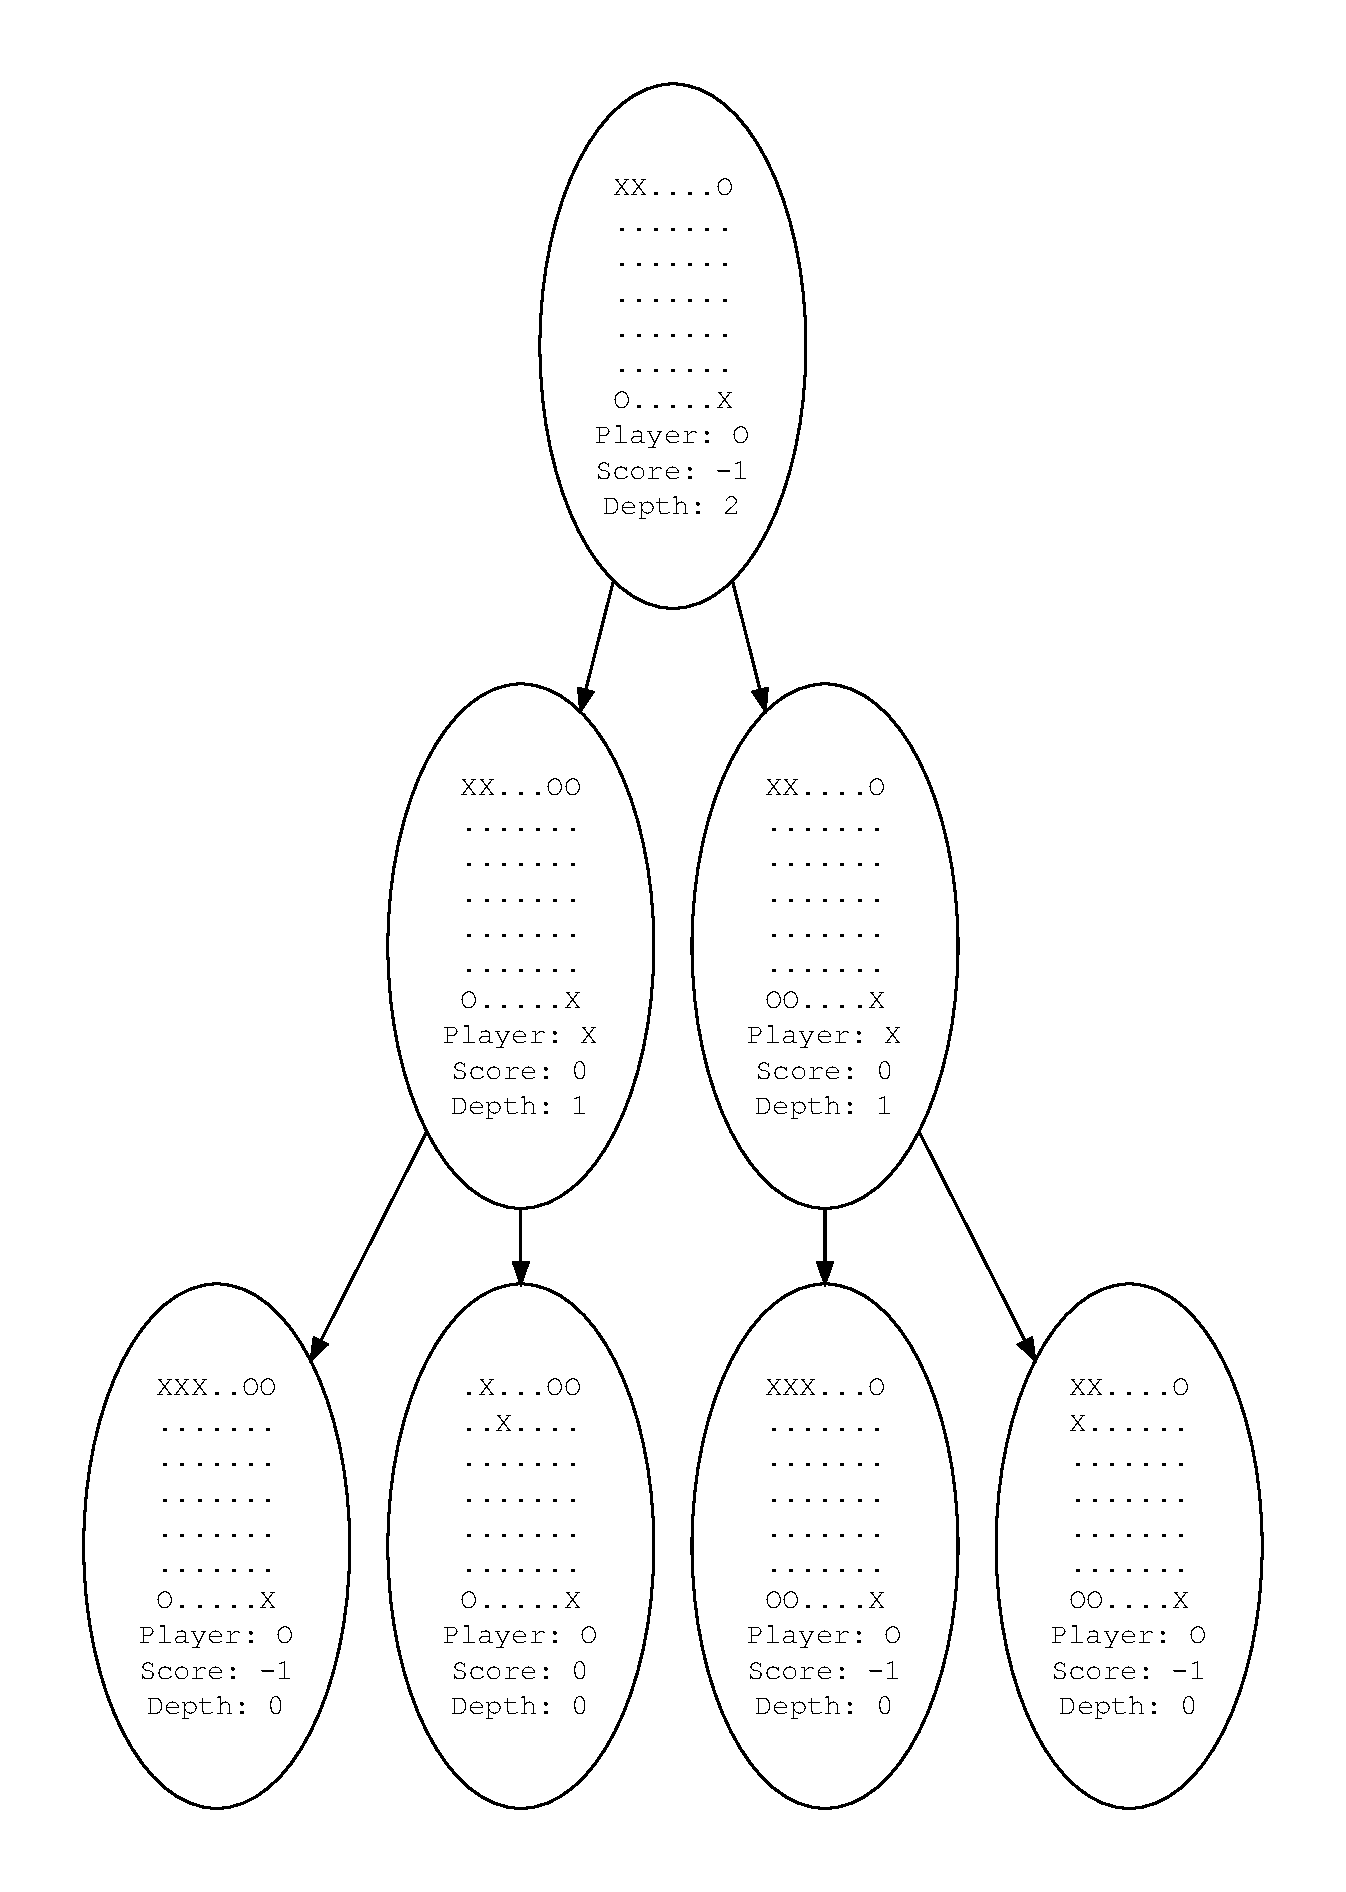
\includegraphics[scale=0.5]{negamax}\end{center}\caption{An example minimax search tree (with many nodes missing).  Depth indicates how many more levels to search for.  In this case, for both nodes of depth 1 the maximum of the negative children's utility of is $1$, so for the root node the maximum of the negative children's utility is $-1$.}\end{figure}

\section{Alpha-beta pruning}
A problem with the na\"ive negamax algorithm is that it can waste a lot of time searching through nodes which are necessarily suboptimal and will not affect the utility calculation.  Alpha-beta pruning \cite{hart} is a method of cutting down the search space while provably not changing the final utility calculated.

For example, if the utility of one child of the root is known to be $-1$, and during searching the utility of another child of the root is shown to be $-1$ or less then this second node and any unexamined nodes beneath it may simply be ignored, since there is no point in considering the second move over the first; it is already known the opponent can force a score $-1$, so that's what they will do (unless there is an even worse score they can force in the examined part). %only way they could be reached is if the opponent made a blunder; i.e., by playing the second node instead of the first.

This is demonstrated in Figure 2, which is a depth 2 search tree with alpha-beta pruning, where the first child node had utility $-1$ and all the remaining child nodes were immediately seen to have utility at most $-1$ or $-2$, so definitely no better than the first child node.  The highlighted nodes show the optimal sequence of moves found for both players (in fact, many of the nodes are in a tie for the optimal move in this case).

\begin{figure}\begin{center}
\includegraphics[scale=0.08]{alphabeta}\end{center}\caption{Depth 2 search tree with alpha-beta pruning, for a response move to \X\ playing the opening move \texttt{b1}.  Each of child nodes of the root (besides the first) only needed one node to be searched beneath them, opposed to the $\approx25$ nodes each had without pruning.}\end{figure}

\section{Results}
Using a search depth of 5 was found to select a move almost instantaneously, while using a search depth of 6 could take around 30 seconds during the middle of the game, when the branching factor is largest.

Using a search depth of 6, \textsl{Ataxx AI} was pitted against the AI from \textsl{The 7th Guest}, and was found to play significantly better, winning the game 35--14.  A record of the complete game is available in appendix A.

\textsl{Ataxx AI} was also tested against \textsl{SlimeWar} \cite{levin}, an open-source Ataxx clone which claims to have beaten all Ataxx AI implementations available online.  It has user-customizable options; they were set to use a maximum search depth of 6 and maximum time of 30 seconds.  \textsl{Ataxx AI} also used a search depth of 6 and ultimately won 27--22.  A record of the complete game is available in appendix B.

\begin{center}\begin{tabular}{c@{\qquad\qquad}c}
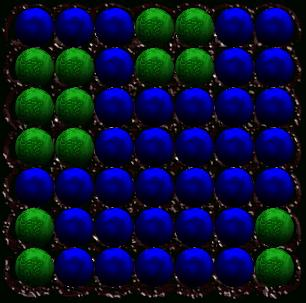
\includegraphics[scale=0.5]{microscope} & 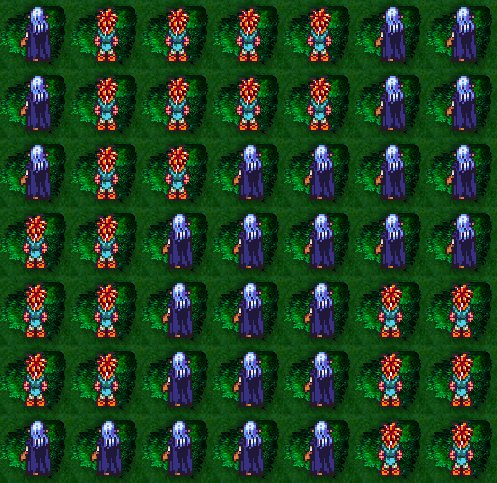
\includegraphics[scale=0.25]{slimewar} \\
\text{Final position against \textsl{The 7th Guest}} & \text{Final position against \textsl{SlimeWar}}
\end{tabular}\end{center}

\begin{thebibliography}{9}
\bibitem{pressibus}Alain Beyrand, \textsl{Ataxx - Origins}. \url{http://www.pressibus.org/ataxx/gen/gborigines.html}
\bibitem{pressibus2}Alain Beyrand, \textsl{Ataxx - The 7th guest - Microscope}. \url{http://pressibus.org/ataxx/dos/gb7thguest.html}
\bibitem{hart}Timothy Hart, Daniel Edwards, \textsl{The Tree Prune (TP) Algorithm}.  Artificial Intelligence Project Memo 30, MIT, 1961.
\bibitem{levin}Michael Levin, \textsl{SlimeWar: An Ataxx Clone}, \url{http://sourceforge.net/projects/slimewar/}
\bibitem{rusnor}Stuart Russell, Peter Norvig, \textsl{Artificial Intelligence: A Modern Approach}, Section 5.2.  Prentice Hall, 1995.
\bibitem{shannon}Claude Shannon, \textsl{Programming a Computer for Playing Chess}.  Philisophical Magazine, 1950.
\end{thebibliography}

\pagebreak
\appendix\section{Versus \textsl{The 7th Guest}}
The following is the game between \textsl{Ataxx AI} (as \X) set to a search depth of 6 and \textsl{The 7th Guest} (as \O).  The final score was 35--14 for my program.
\begin{center}\texttt{X.....O~XX....O~XX...OO~XXX..OO~XXX.OOO~XXXXXOO~XXOOO.O~XXXXO.O~XXXOO.O~\\
.......~.......~.......~.......~.......~.......~...O...~..XX...~..XOO..~\\
.......~.......~.......~.......~.......~.......~.......~.......~.......~\\
.......~.......~.......~.......~.......~.......~.......~.......~.......~\\
.......~.......~.......~.......~.......~.......~.......~.......~.......~\\
.......~.......~.......~.......~.......~.......~.......~.......~.......~\\
O.....X~O.....X~O.....X~O.....X~O.....X~O.....X~O.....X~O.....X~O.....X~\\
~\\
XXXOO.O~XXXOOOO~XXXOOOO~XXXOOOO~XXXOOOO~XXXOOOO~XXXOOOO~XXXOOOO~XXXOOOO~\\
.XXOO..~.XXOO..~XXXOO..~XXXOOO.~XXXOOO.~XXXOOOO~XXXOOOO~XXXOO.O~XXXXX.O~\\
.......~.......~.......~.......~.......~.......~.......~.......~...X...~\\
.......~.......~.......~.......~.......~.......~.......~...O...~...X...~\\
.......~.......~.......~.......~.......~.......~....X..~....O..~....O..~\\
.......~.......~.......~.......~.....X.~.....X.~.....X.~.....X.~.....X.~\\
O.....X~O.....X~O.....X~O.....X~O.....X~O.....X~O.....X~O.....X~O.....X~\\
~\\
XXXO.OO~XXXO.OO~XXXOOOO~XXXOOOO~XXXOOOO~XXXOOOO~XXXO.OO~XXXO.XX~XXXOOOX~\\
XOOOX.O~XXXOX.O~XXXOO.O~XXXOO.O~XXXOO.O~XXXOO.O~XXXOO.O~XXXOXXX~XXXOOOX~\\
..OO...~.XXO...~.XXO...~.XXX...~.XXOO..~.XXXX..~.XXXOO.~.XXXXX.~.XXXXX.~\\
...O...~...O...~...O...~..XX...~..XO...~..XXX..~..XXO..~..X.O..~..X.O..~\\
....O..~....O..~....O..~....O..~.......~.......~.......~.......~.......~\\
.....X.~.....X.~.....X.~.....X.~.....X.~.......~.......~.......~.......~\\
O.....X~O.....X~O.....X~O.....X~O.....X~O.....X~O.....X~O.....X~O.....X~\\
~\\%\pagebreak
XXXOOOX~XXXOOOX~XXXOOOX~XXXOOOX~XXXOOXX~XXXOOXX~XXXOOXX~XXXOOXX~XXXOOXX~\\
XXXOOOX~XXXOOOO~XXXOOOO~XXXOOO.~XXXOOXX~XXXOOXX~XXXOOXX~OOXOOXX~OOXOOXX~\\
.XXXXX.~.XXXXOO~.XXXXXX~.XXXXOO~.XXXXXX~.XXXXXX~.XXXXXX~OOXXXXX~OXXXXXX~\\
..XXX..~..XXX..~..XXXX.~..XXXOO~..XXXOO~..OOO.O~..OOXXX~...OXXX~..XXXXX~\\
.......~.......~.......~.......~.......~...O...~...O...~...O...~...X...~\\
.......~.......~.......~.......~.......~.......~.......~.......~.......~\\
O.....X~O.....X~O.....X~O.....X~O.....X~O.....X~O.....X~O.....X~O.....X~\\
~\\
XXXOOXX~XXXOOXX~XXXOOXX~XXXOOXX~XXXOOXX~XXXOOXX~XXXOOXX~XXXOOXX~XXXOOXX~\\
OOXOOXX~OOXOOXX~OOXOOXX~OOXOOXX~OOXOOXX~OOXOOXX~OOXOOXX~OOXOOXX~OOXOOXX~\\
OOOXXXX~OOOXXXX~OOOXXXX~OOOXXXX~OOOXXXX~OOOXXXX~OOOXXXX~OXXXXXX~OXXXXXX~\\
.OOXXXX~.XXXXXX~.OOXXXX~.OOXXXX~OOOXXXX~XXOXXXX~XX.OOOX~XXXXOOX~XXXXO.X~\\
...X...~..XX...~.OOX...~.XXX...~.OXX...~XXXX...~XXXOO..~XXXXO..~XXXOO..~\\
.......~.......~.......~..X....~..X....~.......~.......~.......~....O..~\\
O.....X~O.....X~......X~......X~......X~......X~......X~......X~......X~\\
~\\\pagebreak
XXXOOXX~XXXOOXX~XXXOOXX~XXXOOXX~XXXOOXX~XXXOOXX~XXXOOXX~XXXOOXX~XXXOOXX~\\
OOXOOXX~OOXOOXX~OOXOOXX~OOXOOXX~OOXOOXX~OOXOOXX~OOXOOXX~OOXOOXX~OOXOOXX~\\
OXXXXXX~OXXXXXX~OXXXXXX~OXXXXXX~OXXXXXX~OXXXXXX~OXXXXXX~OXXXXXX~OXXXXXX~\\
XXXXXXX~XXXXOOO~XXXXOXX~XXXXOXX~XXXXOXX~XXXXOXX~XXXXOXX~XXXXOXX~XXXXOXX~\\
XXXOX..~XXXOOO.~XXXOOXX~XXXOOOO~XXXXXOO~XXXXXOO~XXXXXOO~XXXXXOO~.XXXXOO~\\
....O..~....O..~....O..~....OO.~...XXO.~...OOO.~..XXOO.~..OOOO.~..XXOO.~\\
......X~......X~.......~.......~.......~....O..~....O..~...OO..~..XXO..~\\
~\\
XXXOOXX~XXXOOXX~XXXOOXX~XXXOOXX~XXXOOXX~XXXOOXX~XXXOOXX~XXXOOXX~XXXOOXX~\\
OOXOOXX~OOXOOXX~OOXOOXX~OOXOOXX~OOXOOXX~OOXOOXX~OOXOOXX~OOXOOXX~OOXOOXX~\\
.XXXXXX~.XXXXXX~.XXXXXX~.XXXXXX~OOXXXXX~OOXXXXX~OOXXXXX~OOXXXXX~OOXXXXX~\\
OOXXOXX~OOXXOXX~.OXXOXX~XXXXOXX~OOXXOXX~OOXXOXX~OOXXOXX~OOXXOXX~OOXXOXX~\\
OOXXXOO~XXXXXOO~OOXXXOO~XXXXXOO~XXXXXOO~XXXXXOO~XXXXXOO~XXXXXOO~XXXXX.O~\\
..XXOO.~.XXXOO.~OOXXOO.~OOXXOO.~OOXXOO.~XXXXOO.~XXXXOOO~XXXXXXX~XXOOOXX~\\
..XXO..~..XXO..~..XXO..~..XXO..~..XXO..~.XXXO..~.XXXO..~.XX.XX.~.XOOOX.~\\
~\\
XXXOOXX~XXXOOXX~XXXOOXX~XXXOOXX~XXXOOXX~\\
OOXOOXX~OOXOOXX~OOXOOXX~OOXOOXX~OOXOOXX~\\
OOXXXXX~OOXXXXX~OOXXXXX~OOXXXXX~OOXXXXX~\\
OOXXXXX~OOXXXXX~OOXXXXX~OOXXXXX~OOXXXXX~\\
XXXXXXX~XXXXXXX~XXXXXXX~XXXXXXX~XXXXXXX~\\
XXOOXXX~XXOOXOO~XXOXXXO~OO.XXXO~OXXXXXO~\\
.XOOOX.~.XOO.OO~.XOXXXO~OOOXXXO~OXXXXXO~
}\end{center}

\section{Versus \textsl{SlimeWar}}
The following is the game between \textsl{Ataxx AI} (as \O) and \textsl{SlimeWar} (as \X), both set to search to a depth of 6.  The final score was 27--22 for my program.
\begin{center}\texttt{X.....O~XX....O~XX....O~XX....O~XX....O~XX....O~XX...OO~XX...OO~XX...OO~\\
.......~.......~.......~.......~.......~.......~.......~.......~.......~\\
.......~.......~.......~.......~.......~.......~.......~.......~.......~\\
.......~.......~.......~.......~.......~.......~.......~.....X.~O....X.~\\
.......~.......~.......~.......~O......~O...X..~O...X..~O...X..~O...X..~\\
.......~.......~O......~O....X.~O....X.~O....X.~O....X.~O....X.~O....X.~\\
O.....X~O.....X~O.....X~O.....X~O.....X~O.....X~O.....X~O.....X~O.....X~\\
~\\
XX...OO~XX....O~XX....O~XX....O~XX....O~XX....O~XX....O~XX....O~XX....O~\\
.......~.......~.......~.......~.......~.......~.......~.......~.......~\\
.......~......O~......O~......O~......O~......O~......O~......O~......X~\\
O....X.~O....O.~X....O.~X....O.~X....O.~X...OO.~X...XO.~X...XO.~X....XX~\\
O..XX..~O..XX..~XX..X..~XX..OO.~XX..XX.~XX..OO.~XX.XXO.~OO.XXO.~OO.XXX.~\\
O....X.~O....X.~X....X.~X....O.~X...XX.~X...XX.~X...XX.~OO..XX.~OO..XX.~\\
O.....X~O.....X~O.....X~O.....X~O......~O......~O......~O......~O......~\\
~\\\pagebreak
XX....O~XX....O~XX....O~XX....O~XX....O~XX....O~XX....O~XX....O~XX....O~\\
.......~.......~.......~.......~.......~.......~.......~.......~.......~\\
......X~......X~......X~.......~.......~.X.....~.X.....~.X.....~.O.....~\\
X....XX~X....XX~X....OO~X...XXO~OO..XXO~XX..XXO~XX..XXO~X...XXO~OO..XXO~\\
O..OOX.~XX.OOX.~XX.OOOO~XX.XXXO~OO.XXXO~OO..XXO~OO..XXO~OX..XXO~OO..XXO~\\
OO.OOX.~XX.OOX.~XX.O.O.~XX.O.O.~XX...O.~XX...O.~OO...O.~OXX..O.~OXX..O.~\\
O......~O......~O......~O......~O......~O......~OO.....~OX.....~OX.....~\\
~\\
.X....O~.X....O~.X....O~.X....O~.X....O~.X....O~.X....O~.X....O~.X....O~\\
.......~.......~.......~.......~.......~.......~.......~.......~.......~\\
XX.....~XX.....~XX.....~XX.....~XX.....~XX.....~XX.....~XX.....~XX.....~\\
XX..XXO~XX..XXO~XX...XO~XX...XO~XX...XO~XX...XO~XX...XO~XX...OO~XX...XO~\\
OO..XXO~OO..OOO~OO..OXX~OO...XX~OXX..XX~OXX..XX~OXX...X~OXX..OO~OX..XXO~\\
OXX..O.~OXX.OO.~OXX.OXX~OOO.OXX~OXX.OXX~OXX..OO~OXX..XX~OXX..OO~OXX..XO~\\
OX.....~OX.....~OX.....~OOO....~OOO....~OOO...O~OOO..XX~OOO..XX~OOO..XX~\\
~\\
.X....O~.X....O~.X....O~.X....O~.X....O~.X....O~.O....O~.X....O~.X....O~\\
.......~.......~.......~.......~.......~.......~..O....~.XX....~.OO....~\\
XX.....~XX.....~XX.....~XX.....~XO.....~XO.....~XO.....~XX.....~XOO....~\\
XX..OO.~XX..OO.~XX..OO.~XX..OXX~XOO..XX~XXX..XX~XXX..XX~XX...XX~XO...XX~\\
OX..OOO~OX..XXO~OX..XXO~OX..XXX~OO..XXX~OXX.XXX~OXX.XXX~OXX.XXX~.XX.XXX~\\
OXX..XO~OX..XXO~OX..OOO~OX..OOO~OX..OOO~OX..OOO~OX..OOO~OX..OOO~OX..OOO~\\
OOO..XX~OOO..XX~OO..OOX~OO..OOX~OO..OOX~OO..OOX~OO..OOX~OO..OOX~OO..OOX~\\
~\\
.X....O~.X....O~.X....O~.O....O~.O....O~.O....O~.XX...O~OOX...O~OOX...O~\\
.OO....~.OO....~.OO....~OOO....~OOX....~OOX....~OXX....~OOX....~OOX....~\\
XOO....~XOO....~XOO....~OOO....~OOXX...~OOXX...~OOX....~OOX....~OOX....~\\
XX...XX~XOO..XX~XOO..XX~XOO..XX~XOX..XX~XOX..XX~XOX..XX~XOX..XX~XOX..XX~\\
XXX.XXX~XOO.XXX~XXX.XXX~XXX.XXX~XXX..XX~XXX..XX~XXX..XX~XXX..XX~XX...XX~\\
XX..OOO~XX..OOO~XXX.OOO~XXX.OOO~XXX.OOO~XOO..OO~XOO..OO~XOO..OO~XOO.XXO~\\
OO..OOX~OO..OOX~OX..OOX~OX..OOX~OX..OOX~OOO.OOX~OOO.OOX~OOO.OOX~OOO.XXX~\\
~\\
OOX...O~OOX...O~OOO...O~OOO...O~OOO...O~OOO...O~OOOO..O~OOOXX.O~OOOXX.O~\\
OOX....~OOX....~OOOO...~OOXX...~OOXX...~OOXX...~OOOO...~OOOX...~OOOX...~\\
OOX....~OOX....~OOO....~OOXX...~OOXX...~OOXX...~OOXX...~OO.X...~OO.X...~\\
XOX..OX~XOX..OX~XOX...X~XOX...X~XOX..OO~XO...OO~XO...OO~XO...OO~XO...OO~\\
XX..OOX~XX..OXX~XX..OXX~XX..OXX~XX..OOO~XX..XOO~XX..XOO~XX..XOO~XOO.XOO~\\
XOO.OO.~XOO.OXX~XOO.OXX~XOO.OXX~XOO.OXX~XOXXXXX~XOXXXXX~XOXXXXX~XOOOXXX~\\
OOO.XXX~OOO.XXX~OOO.XXX~OOO.XXX~OOO.XXX~OOX.XXX~OOX.XXX~OOX.XXX~OOX.XXX~\\
~\\\pagebreak
OOOXX.O~OOOXX.O~OOOXX.O~OOOXX.O~OOOXX.O~OOOXX.O~OOOXX.O~OOOOO.O~OOOOO.O~\\
OXXX...~OXXX...~OXXX...~OXXX...~OXXX...~OXXX...~OXX....~OXOO...~OXXX...~\\
OXXX...~OXXX...~OXX....~OXX....~OXX....~OXO....~OXO....~OXO....~OXXX...~\\
XX...OO~XX...OO~XX...OO~XX...OO~XXX..OO~XXOO.OO~XXOXXXO~XXOXXXO~XXXXX.O~\\
XOO.XOO~X.O.XOO~XXX.XOO~XXOOOOO~XXXXOOO~XXOOOOO~XXOXXXO~XXOXXXO~XXOXXXO~\\
XOOOXXX~XOOOOXX~XXXOOXX~XXOOOXX~XXOOOXX~XXOOOXX~XXOOOXX~XXOOOXX~XXOOOXX~\\
OOX.XXX~OOOOOXX~OOOOOXX~OOOOOXX~OOOOOXX~OOOOOXX~OOOOOXX~OOOOOXX~OOOOOXX~\\
~\\
OOOOO.O~OOOOO.O~OOOOO.O~OOOXX.O~OOOXO.O~OOO.O.O~OOOOO.O~OOOOXXX~OOOOXXX~\\
OXXX...~OXXX...~OXXX...~OXXXX..~OXXXOO.~OXXXXX.~OXOOOX.~OXOOXX.~OXOOXX.~\\
OXXX...~OXXXX..~OXXXX..~OXXXX..~OXXXO..~OXXXXX.~OXXXXX.~OXXXXX.~OXXXOO.~\\
XXXXOOO~XXXXXXO~XXOOOXO~XXOOO.O~XXOOO..~XXOOX..~XXOOX..~XXOOX..~XXOOOO.~\\
XXOXOOO~XXO.OOO~XXOOOOO~XXOOOOO~XXOOOOO~XXOOOOO~XXOOOOO~XXOOOOO~XXOOOOO~\\
XXOOOXX~XXOOOXX~XXOOOXX~XXOOOXX~XXOOOXX~XXOOOXX~XXOOOXX~XXOOOXX~XXOOOXX~\\
OOOOOXX~OOOOOXX~OOOOOXX~OOOOOXX~OOOOOXX~OOOOOXX~OOOOOXX~OOOOOXX~OOOOOXX~\\
~\\
OOOOXXX~OO.OOOX~OXXXOOX~OXXXO.X~OXX.XXX~OXX.XOO~OXXXXOO\\
OXOO.X.~OXOOOO.~OXXXOO.~OXXXOO.~OXXXXX.~OXXXXOO~OXXXXOO\\
OXXXOX.~OXXOOO.~OXXOOO.~OXXOOOO~OXXOOOO~OXXOOOO~OXXOOOO\\
XXOOOXX~XXOOOXX~XXOOOXX~XXOOOOO~XXOOOOO~XXOOOOO~XXOOOOO\\
XXOOOXX~XXOOOXX~XXOOOXX~XXOOOXX~XXOOOXX~XXOOOXX~XXOOOXX\\
XXOOOXX~XXOOOXX~XXOOOXX~XXOOOXX~XXOOOXX~XXOOOXX~XXOOOXX\\
OOOOOXX~OOOOOXX~OOOOOXX~OOOOOXX~OOOOOXX~OOOOOXX~OOOOOXX
}\end{center}

\end{document}
